%\setcounter{chapter}{33}
\chapter{Conditional Generative Models}\label{chapter:conditional_generative_models}

\index{Generative models|Conditional}

\section{Introduction}

In the preceding chapters, we learned about two uses of generative models: (1) as a way to synthesize realistic but novel data, and (2) as a way to learn representations of the data. Now we will introduce a third use, which is arguably the most widespread use of generative models: \textit{as a way to solve prediction problems}.

\section{A Motivating Example: Image Colorization}

To motivate this use case, consider the following problem. We wish to colorize a black and white photo, that is, we wish to predict the color of each pixel in a black and white photo.

Now, we already have seen some tools we could apply to this problem. First we will try to solve it with least-squares regression. Second, with softmax classification. We will see that both approaches fall short of a good solution. This will motivate the necessity of conditional generative models, which turn out to solve the colorization problem quite nicely, and can produce nearly photorealistic results.

\subsection{The Failure of Point Prediction: Multimodal Distributions}

We could formulate the problem as least-squares regression: train a function to output a vector of real-valued numbers, representing the red, green, and blue values of every pixel in the image, then penalize the squared distance between these values and the ground truth values.

This kind of regression fits a function $f: \mathcal{X} \rightarrow \mathcal{Y}$. For every input $\mathbf{x} \in \mathcal{X}$, the output is a single \index{Point prediction}\textbf{point prediction} $\hat{\mathbf{y}} \in \mathcal{Y}$, that is, we output just a \textit{single} prediction of what the value of $\mathbf{y}$ should be.

% figure of point prediction

\begin{figure}
    \centerline{
        \begin{minipage}{0.15\linewidth}
            \begin{tikzpicture}
                \node[] (image) at (0,0) {\includegraphics[width=0.75\linewidth]{./figures/conditional_generative_models/cgen_tshirts_obs.pdf}};
                \draw (0,-1) node {Observation};
            \end{tikzpicture}
            \vspace{-0.2cm}
        \end{minipage}
        \hfill
        \begin{minipage}{0.84\linewidth}
            \begin{subfigure}[b]{0.5\textwidth}
                \includegraphics[width=1.0\linewidth]{./figures/conditional_generative_models/cgen_tshirts_gt.pdf}
                \caption*{(a) True data distribution}
                \vspace{0.4cm}
            \end{subfigure}
            \hfill
            \begin{subfigure}[b]{0.5\textwidth}
                \includegraphics[width=1.0\linewidth]{./figures/conditional_generative_models/cgen_tshirts_point.pdf}
                \caption*{(b) Point prediction (regression)}
                \vspace{0.4cm}
            \end{subfigure}
            \hfill
            \begin{subfigure}[b]{0.5\textwidth}
                \includegraphics[width=1.0\linewidth]{./figures/conditional_generative_models/cgen_tshirts_gauss.pdf}
                \caption*{(c) Gaussian}
            \end{subfigure}
            \hfill
            \begin{subfigure}[b]{0.5\textwidth}
                \includegraphics[width=1.0\linewidth]{./figures/conditional_generative_models/cgen_tshirts_class.pdf}
                \caption*{(d) Softmax (classification)}
            \end{subfigure}
            \hfill
        \end{minipage}
    }
    \caption{Different kinds of predictive distributions.}
    \label{fig:conditional_generative_models:tshirts}
\end{figure}

What if there are multiple equally valid answers? Taking a color image and making it grayscale is a many-to-one mapping: for any given grayscale value, there are many different color values that could have projected to that value of gray. This means that the colorization problem is fundamentally ambiguous, and there may be multiple valid color solutions for any grayscale input. A point estimate is bound to be a poor inference in this case, since a point estimate can only predict one of the multiple possible solutions.

%In psychology, the word for two \textit{different} physical signals that are perceived as the \textit{same} is \textbf{metamers}. Two t-shirts that are different colors but appear the same in black-and-white are metamers w.r.t. the color-to-grayscale transformation. If you see some shade of gray on the shirt, it is impossible to know which of the metameric colors produced that shade. Metamers are ubiquitous in perception, and they are the defining property of ``inverse problems", which are problems of inverting a many-to-one mapping. For these problems, a point estimate is bound to be a poor inference, since a point estimate can only predict one of the multiple possible solutions.

% figure of colorizing a bird with least-squares (can use a result from CIC)

Figure \ref{fig:conditional_generative_models:tshirts} shows several kinds of predictions one could make given an observation of a grayscale t-shirt. The question is straightforward: What is the color of the shirt? To unify different kinds of prediction models, we will represent them all as outputting a distribution over the possible colors of the shirt. Let $A$ be a random variable that represents the $a$ value of the shirt in $lab$ color space. Our input is just the $l$ value of the shirt. Our predictions will be represented as $p_{\theta}(A \given l)$. The particular shirt we are looking at comes in two colors, either teal or pink. The true data distribution, $p_{\texttt{data}}$, is therefore two delta functions, one on teal and the other on pink.

Least-squares regression results in a model that predicts the \textit{mean} of the data distribution. Therefore, the point prediction output by a least-squares regressor will be that the shirt is gray. The probability density associated with this prediction is shown in \fig{\ref{fig:conditional_generative_models:tshirts}}(b).\marginnote{A point prediction does not necessarily come with probabilistic semantics, but here we will interpret a prediction of $\hat{a} = f_{\theta}(l)$ as implying a predictive distribution over $A$ that has the form $p_{\theta}(A = a \given l) = \delta(a - \hat{a})$, where $\delta$ is the Dirac delta function.}

This prediction is entirely wrong! It splits the difference between the two true possibilities and comes out with something that has \textit{zero} probability under the data distribution. As discussed in \chap{\ref{chapter:probabilistic_graphical_models}}, we could have done regression with a different loss function (using the $L_1$ loss for example, rather than $L_2$), and we would have come up with a different solution. But we will never get the correct solution. Because the true distribution has two equally probable modes, and a single point prediction can only ever represent one mode.

We can do better by predicting a \textit{distribution} rather than a point estimate. An example is shown in \fig{\ref{fig:conditional_generative_models:tshirts}}(c), where we predict a Gaussian distribution. In fact, the least-squares regression model can be described as outputting the mean of a max likelihood Gaussian fit to $p_{\theta}(A \given l)$. Predicting the distribution then just requires also predicting the variance of the Gaussian. This gives us a better sense of the possible colors the shirt could be, but it is still a unimodal distribution, while the data is bimodal.

Naturally, then, we may want to predict a more expressive distribution; a mixture of two Gaussians could, for example, capture the bimodal nature of the data. An easy way to predict a distribution is to predict the parameters of some parametric family of distributions. This is precisely what we did with the Gaussian fit: the parameters of a 1D Gaussian are its mean and variance, so if $\hat{\mathbf{y}} \in \mathbb{R}^2$ then $\hat{\mathbf{y}}$ suffices to parameterize a 1D Gaussian. A mixture of $N$ Gaussians just requires outputting $3N$ numbers: the mean, variance, and weight of each Gaussian in the mixture. The loss function could then just be the data likelihood under the mixture of Gaussians parameterized by $\hat{\mathbf{y}} \in \mathbb{R}^{3N}$.

One of the most common choices for an expressive, multimodal family of distributions is the categorical distribution, $\texttt{Cat}$. This distribution applies only to discrete random variables, so to use it, the first thing we have to do is quantize our possible output values. \Fig{\ref{fig:conditional_generative_models:tshirts}}(d) shows an example, where we have quantized the $a$-value into ten bins. Then the categorical distribution is simply a ten-dimensional vector of nonnegative numbers that sum to 1 (i.e., a probability mass function). The nice thing about this parameterization is that \textit{all} probability mass functions over $k$ classes are members of the family $\texttt{Cat}(k)$. In other words, this is the most expressive distribution possible over a discrete random variable! That's great because it means we can use it to represent predictions with any number of modes (well, up to $k$, the resolution of our quantized data).

In fact, we have already seen one super important use of the categorical distribution: \textit{softmax regression} (\sect{\ref{sec:intro_to_learning:image_classification}}). Now you might have a better understanding of why classification is such a ubiquitous modeling tool: it models a maximally expressive predictive distribution over a quantized decision space.\marginnote{Remember that softmax \textit{regression} is a way to solve a \textit{classification} problem. It is called regression since we predict a set of continuous numbers (a probability distribution), then take the argmax of this set to perform the classification.}[-0.4cm]

\subsection{Classification to the Rescue?}

Classification solves some of the deficiencies of point prediction. However, it comes with several new problems of its own:
\begin{itemize}
    \item It incurs quantization error.
    \item It may require a number of classes exponential in the data dimensionality.
\end{itemize}
The first is not such a big issue. You can see its effect in \fig{\ref{fig:conditional_generative_models:tshirts}}(d). The true colors are teal and bright pink but the quantization lowers the color resolution and we cannot know if the prediction is that the shirt is dull pink or bright pink as both fall in the same bin. This is why the pink shirt here appears slightly duller than in the data distribution (we colored each bin with the floor of its range). But generally this isn't such a big deal. We can always increase the resolution by increasing $k$. Most image formats only represent 256 possible values for $a$, so if we set $k=256$ then we incur no quantization error.\marginnote{Why 256 values? Because each channel in standard image formats is stored as an array of \texttt{uint8}s.}[-0.5cm]

The second issue is much more severe. If we are predicting the $a$-value of a single pixel, then the classification approach says there are $k$ possible values it could take on. This approach can be extended to predicting $ab$-values: we come up with a list of discrete color classes, like \texttt{red}, \texttt{orange}, \texttt{turquoise}, and so forth. But to tile the two-dimensional space of $ab$-values will require $k^2$ color classes, if we wish to retain a resolution of $k$ for both $a$ and $b$. Nonetheless, we can still do this using a reasonable number of classes, and it might look like as shown in \fig{\ref{fig:conditional_generative_models:color_quantization}}.
\begin{figure}[h!]
    \centerline{
        \includegraphics[width=0.8\linewidth]{./figures/conditional_generative_models/color_quantization.pdf}
    }
    \caption{The funny shape of the $lab$ color gamut is because not every $ab$ value maps to a valid pixel color. When working with predictions over $lab$ color space, we may map $ab$ values that fall outside the gamut (valid range) to the nearest in-gamut value.}
    \label{fig:conditional_generative_models:color_quantization}
\end{figure}

The real problem comes about when predicting more than one pixel. To quantize the $ab$-values of $N$ pixels requires $k^{2N}$ classes, again assuming we want a resolution of $k$ for the $a$ and $b$ value of each pixel. For a $256 \times 256$ resolution image, the number of classes required is astronomical (for $k=10$, the number is a one followed by over 100,000 zeros).\marginnote{Quantizing on a grid doesn't scale to high-dimensions, but more intelligent quantization methods can work. These more intelligent methods are called \textbf{vector quantization} or \textbf{clustering}, and we cover them in \chap{\ref{chapter:representation_learning}}.}[-3.6cm]

\subsection{The Failure of Independent Predictions: Joint Structure}

To circumvent this curse of dimensionality, we can turn to factorization: rather than treating the whole configuration of pixels as a class, make \textit{independent} predictions for each pixel in the image. From a probabilistic inference perspective, the corresponds to the following factorization of the joint distribution:
\begin{align}
    p_{\theta}(\mathbf{ab} \given \mathbf{l}) = \prod_{n=1}^N\prod_{m=1}^M  p_{\theta}(ab[n,m,:] \given \mathbf{l})
\end{align}
\marginnote{Note the similarity between this image model and the ``independent pixels'' model we saw in \eqn{\ref{eq:histmodel}} in \chap{\ref{chapter:stat_image_models}}. The present model can represent images with more structure because rather than assuming the pixels are all completely independent (i.e., marginally independent), it only assumes the pixel colors are \textit{conditionally} independent, conditioned on the luminance image (which provides a great deal of structure).}[-0.8cm]
The underlying assumption of this factorization is one of conditional independence: each pixel's $ab$ value is considered to be conditionally independent from all other pixels' $ab$ values, given the observed luminance (of all pixels). This is a very common assumption in image modeling problems: in fact, \textit{whenever} you use least-squares regression for a multidimensional prediction, you are implicitly making this same assumption. To see this, suppose you are predicting a vector $\mathbf{y}$ from an observed vector $\mathbf{x}$, and your prediction is $\hat{\mathbf{y}} = f(\mathbf{x})$. Then, we can write the least-squares objective ($L_2$) as:
\begin{align}
    -\norm{\hat{\mathbf{y}} - \mathbf{y}}^2_2 & = \sum_i -(\hat{y}_i - y_i)^2      \\
                                              & = \log \prod_i \phi(\hat{y}_i,y_i)
\end{align}
The loss factorizes as a product over pairwise potentials. Therefore, by the Hammersley-Clifford theorem (\chap{\ref{chapter:probabilistic_graphical_models}}), the $L_2$ loss implies a probability distribution that treats all true values $y_i$ as independent from one another, given all the predictions $\hat{y}_i$. The predictions are a function of just the input $\mathbf{x}$, so the implication is that all the true values $y_i$ are independent from one another given the observation $\mathbf{x}$. Therefore, we have arrived at our conditional independence assumption: each dimension's predicted value is assumed to be independent of each other dimension's predicted values, given the observed input. This is a huge assumption and rarely true of prediction problems in computer vision!

%Notice that $\phi = e^{-(\hat{y}_i - y_i)^2}$ is a non-negative function, which means we can interpret it as an unnormalized probability density over the event $\{y_i, \hat{y}_i\}$. 

%which equals $p(y_i | \mathbf{x})$ since $\hat{y}_i$ is a deterministic function of $\mathbf{x}$. From basic probability we know that iff $p(A,B | C) = p(A | B)p(A | C)$ then $A$ and $B$ are conditionally independent given $C$.

%Therefore, we have that:
%\begin{align}
%    \argmax_{\hat{\mathbf{y}}} -\norm{\hat{\mathbf{y}} - \mathbf{y}}^2_2 &= %\argmax_{\hat{\mathbf{y}}} \log \prod_i p(y_i|\mathbf{x})
%\end{align}

% need better explanation here, relating to graphical models

So, whether you are using per-pixel classification, or least-squares regression, you are implicitly fitting a model that assumes independence between all the output pixels, conditioned on the input. This is called \index{Unstructured prediction}\textbf{unstructured prediction}.

This causes problems. Let's return to our t-shirt example. We will use a per-pixel color classifier and see where it fails. Since the data distribution has two equally probable modes—teal and pink—the classifier will learn to place roughly equal probability mass on these two modes. As training data and time go to infinity, the classifier should recover the exact data distribution, but with finite data and time it will only be approximate, and so we might have a case where for some luminance values the classifier places 51 percent chance on teal and for others it places 49 percent on teal. Then if, as we scan across pixels in the shirt we are observing, the luminance changes very slightly, the model predictions might wiggle back and forth between 49 percent and 51 percent teal. As our application is to colorize the photo, at some point we need to make a hard decision and output a single color for each pixel. Doing so in the present case will cause chaotic transitions from predicting pink (where $p(\text{teal}) < 0.5$) and teal (where $p(\text{teal}) > 0.5$). An example of this kind of prediction flipping is shown in \fig{\ref{fig:conditional_generative_models:cgen_tshirt_color_inconsistency}}.

% figure of colorizing bird with independent predictions per-pixel (can use a result from CIC)

\begin{figure}[t!]
    \centering
    \includegraphics[width=1.0\linewidth]{./figures/conditional_generative_models/cgen_tshirt_color_inconsistency.pdf}
    \caption{Color flipping can arise from a smooth underlying predictive distribution, on top of which independent choices are made.}
    \label{fig:conditional_generative_models:cgen_tshirt_color_inconsistency}
\end{figure}

\marginnote{
    A real example of color flipping from \cite{zhang2016colorful}. The model is unsure whether the shirt, and the background, are blue or red, so it chaotically alternates between these two options.\\[6pt]
    \centerline{
        \includegraphics[width=.5\linewidth]{./figures/conditional_generative_models/color_flipping_cic.jpg}}
}[-4cm]

%\paragraph{What distinguishes conditional generative models from other kinds of prediction?} 
%What's a data prediction problem: any problem where the thing you want to predict is ``data". Some other important properties associated with generative models are that the predictions parameterize an expressive family of distributions (generally we want ``multimodal" distributions in this family, i.e. probability distributions that have more than one peak).

%\marginnote{In truth, all probabilistic models are generative models. An image classifier is a generative model of one-hot labels, and a linear regression is a generative model of real-valued predictions. But normally we reserve the the term ``generative model" just for cases where the thing we are synthesizing looks like raw data, i.e. pixels, waveforms, character strings, etc.}

%\section{Class-conditional models}
%Chapter \ref{chapter:generative_models} already covered one kind of conditional generative model: 

\section{Conditional Generative Models Solve Multimodal Structured Prediction}

%Chapter \ref{chapter:generative_models} described how generative models can be used to model the joint structure of an entire configuration of many pixels, and can also synthesize a distribution of possibilities. In that chapter we mentioned that the modeled distribution can be either conditional or unconditional, but then focused just on unconditional models. Now we turn our attention to conditional distributions, and see how they can be thought of as solving multimodal structured prediction problems.

In the previous section, we learned that standard approaches to prediction are insufficient for making the kinds of predictions we usually care about in computer vision.

Conditional generative models are a general family of prediction methods that:
\begin{itemize}
    \item Model a multimodal distribution of predictions, and
    \item Model joint structure.
\end{itemize}

Methods that model joint structure in the output space are called \index{Structured prediction}\textbf{structured prediction} methods—they don't factorize the output into independent potentials conditioned on the input. Conditional generative modeling is a structured prediction approach that models a full distribution of possibilities over the joint configuration of outputs.

\subsection{Relationship to Conditional Random Fields}
The conditional random fields (CRFs) from \chap{\ref{chapter:probabilistic_graphical_models}} are one kind of model that fits this definition. Now we will see some other ones. The big difference is that CRFs make predictions via \textit{thinking slow}~\cite{kahneman2011thinking}: given a query observation, you run belief propagation or another iterative inference algorithm to arrive at a prediction. The conditional generative models we will see in this section \textit{think fast}: they do inference through a single forward pass of a neural net. Sometimes the thinking fast approach is referred to as \index{Amortized inference}\textbf{amortized inference}, where the idea is that the cost of inference is amortized over a training phase. This training phase learns a direct mapping from inputs to outputs that approximates the solution we would have gotten if we did exact inference on that input.


\section{A Tour of Popular Conditional Models}
We saw a bunch of unconditional generative models in the previous chapters. How can we make each conditional? It is usually pretty straightforward. This is because if you can model an arbitrary distribution over a random variable, $p(Y)$, then you can certainly model the conditional distribution $p(Y \given X=\mathbf{x})$—it's just another arbitrary distribution. Of course, we typically care about modeling $p(Y \given X=\mathbf{x})$ for \textit{all} possible settings of $\mathbf{x}$. We could, but don't want to, fit a separate generative model for each $\mathbf{x}$. Instead we want neural nets that take a query $\mathbf{x}$ as input and produce an output that models or samples from $p(Y \given X=\mathbf{x})$. We will briefly cover how to do this for several popular models:
\marginnote{In this chapter, $Y$ is the image we are generating and $X$ is the data we are conditioning on. Note that this is different than in the previous generative modeling chapters (\chaps{\ref{chapter:generative_models}} and \ref{chapter:generative_modeling_and_representation_learning}), where $X$ was the image we were generating, unconditionally.}[-3.2cm]

% can we make a table for this?

\subsection{Conditional Generative Adversarial Networks}
\index{Generative adversarial network!Conditional}
We can make a generative adversarial network (GAN; \sect{\ref{sec:generative_models:GANs}}) conditional simply by adding $\mathbf{x}$ as an input to both the generator and the discriminator:
\begin{align}
    \arg\min_{\theta}\max_{\phi} \mathbb{E}_{\mathbf{z},\mathbf{x},\mathbf{y}} \big[ \log d_{\phi}(\mathbf{x}, g_{\theta}(\mathbf{x},\mathbf{z})) + \log (1 - d_{\phi}(\mathbf{x}, \mathbf{y})) \big]
\end{align}
What this does is change the job of the discriminator from asking ``is the output real or synthetic?'' to asking ``is the input-output \textit{pair} real or synthetic?'' An input-output pair can be considered synthetic for two possible reasons:
\begin{enumerate}
    \item The output looks synthetic.
    \item The output does not match the input.
\end{enumerate}
If both reasons are avoided, then it can be shown that the produced samples are $iid$ with respect to the true conditional distribution of the data $p_{\texttt{data}}(Y \given \mathbf{x})$ (this follows from the analogous proof for unconditional GANs in \cite{goodfellow2014generative}, since that proof applies to modeling any arbitrary distribution over $Y$, including $p_{\texttt{data}}(Y \given \mathbf{x})$ for any $\mathbf{x}$).

%One popular class of conditional GAN models solve a problem known as \textbf{image-to-image translation}.

\subsection{Conditional Variational Autoencoders}\label{sec:conditional_generative_models:cVAE}
\index{Variational autoencoder!Conditional}

Recall that a variational autoencoder (VAE; \sect{\ref{sec:generative_modeling_and_representation_learning:VAEs}}) is an infinite mixture model which makes use of the following identity:
\begin{align}
    p_{\theta}(\mathbf{x}) = \int_{\mathbf{z}} p_{\theta}(\mathbf{x} \given \mathbf{z})p_{\mathbf{z}}(\mathbf{z})d\mathbf{z}
\end{align}
Analogously, we can define any conditional distribution as the marginal over some latent variable:
\begin{align}
    p_{\theta}(\mathbf{y} \given \mathbf{x}) = \int_{\mathbf{z}} p_{\theta}(\mathbf{y} \given \mathbf{z}, \mathbf{x})p_{\mathbf{z}}(\mathbf{z} \given \mathbf{x})d\mathbf{z}
\end{align}
In \textbf{conditional VAEs} (\textbf{cVAEs}), we restrict our attention to latent variables $\mathbf{z}$ that are independent of the inputs we are conditioning on, so we have:
\begin{align}
    p_{\theta}(\mathbf{y} \given \mathbf{x}) = \int_{\mathbf{z}} p_{\theta}(\mathbf{y} \given \mathbf{z}, \mathbf{x})p_{\mathbf{z}}(\mathbf{z})d\mathbf{z} \quad\quad \triangleleft \quad\text{cVAE likelihood model}
\end{align}\marginnote{This corresponds to this graphical model:\\
    \medbreak
    \centering
    \includegraphics[width=0.15\linewidth]{./figures/conditional_generative_models/graphical_model_x_z_to_y.pdf}
}[-2.1cm]
The idea is that $\mathbf{z}$ should only encode bits of information about $\mathbf{y}$ that are \textit{independent} from whatever $\mathbf{x}$ already tells us about $\mathbf{y}$. For example, suppose that we are trying to predict the motion of a billiard ball bouncing around in a video sequence. We are given a single frame $\mathbf{x}$ and asked to predict the next frame $\mathbf{y}$. Only knowing $\mathbf{x}$ we can't know whether the ball will move up, down, diagonally, and so on, but we \textit{can} know what color the ball will be in the next frame (it must be the same as the previous frame) and the rough position on the screen of the ball (it can't have moved too far). Therefore, the only missing information about $\mathbf{y}$, given we know $\mathbf{x}$, is the velocity of the ball. Naturally, then, if the model learns to interpret $\mathbf{z}$ as coding for velocity, we would have a perfect prediction $p_{\theta}(\mathbf{y} \given \mathbf{z}, \mathbf{x})$ (one that places max likelihood on the observed next frame $\mathbf{y}$), and marginalizing over all the possible $\mathbf{z}$ values would place max likelihood on the data ($p_{\theta}(\mathbf{y} \given \mathbf{x})$). This is what ends up happening in a cVAE (or, to be precise, it is one solution that maximizes the cVAE objective; it is not guaranteed to be the solution that is arrived at, but it is a good model of what tends to happen in practice). \Fig{\ref{fig:conditional_generative_models:cVAE_ball_bouncing_example}} shows this scenario.
\begin{figure}[h!]
    \centerline{
        \includegraphics[width=0.6\linewidth]{./figures/conditional_generative_models/cVAE_ball_bouncing_example.pdf}
    }
    \caption{A scenario where a yellow ball is moving across a plane. The observation, $\mathbf{x}$, is a static frame. From that observation, we know what will be the color and rough position of the ball in the next frame, $\mathbf{y}$, but we don't know what direction it will have moved, because the velocity of the ball is unobserved. Therefore, velocity is a latent variable and one solution to the cVAE objective will be to encode in the model's latent variables ($\mathbf{z}$) the velocity of the ball, as is depicted here.}
    \label{fig:conditional_generative_models:cVAE_ball_bouncing_example}
\end{figure}

Just like regular VAEs, cVAEs also have an encoder, which acts to predict the optimal importance sampling distribution $p_{\theta}(Z \given \mathbf{x}, \mathbf{y})$. In practice, this means that a cVAE can be trained just like a regular VAE except that the encoder takes the conditioning information, $\mathbf{x}$, as input (in addition to $\mathbf{y}$), and the decoder also takes in $\mathbf{x}$ (in addition to $\mathbf{z}$). Figure \ref{fig:conditional_generative_models:cVAE_ball_bouncing_example_nets} depicts this setting.
\begin{figure}[h!]
    \centerline{
        \includegraphics[width=0.9\linewidth]{./figures/conditional_generative_models/cVAE_ball_bouncing_example_nets.pdf}
    }
    \caption{cVAE architecture. The dotted lines indicate that the \textit{target encoder} is only used during training; at test time, usage follows the solid path.}
    \label{fig:conditional_generative_models:cVAE_ball_bouncing_example_nets}
\end{figure}

%\paragraph{VAEs} To make a VAE conditional, just let the decoder look at $\mathbf{x}$. Then the %encoder will learn to just encode into $\mathbf{z}$ the information about %$\mathbf{y}$ that is not given by $\mathbf{x}$.

\subsection{Conditional Autoregressive Models}
\index{Autoregressive model!Conditional}
Autoregressive models (\sect{\ref{sec:generative_models:autoregressive}}) are already modeling a sequence of conditional distributions. So, to condition them on some inputs $\mathbf{x}$, we can simply concatenate $\mathbf{x}$ as a prefix to the sequence of $y$ values we are modeling, yielding the new sequence: $[x_1, \ldots, x_m, y_1, \ldots, y_n]$. The probability model factorizes as:
\begin{align}
    p_{\theta}(\mathbf{y} \given \mathbf{x}) & = \prod_{i=1}^n p_{\theta}(y_i \given y_1, \ldots, y_{i-1}, x_1, \ldots, x_m)
\end{align}
Each distribution in this product is a prediction of the next item in a sequence given the previous items, which is no different than what we had for unconditional autoregressive models. Therefore, the tools for modeling unconditional autoregressive distributions are also appropriate for modeling conditional autoregressive distributions. From an implementation perspective, the same exact code will handle both cases, just depending on whether you prefix the sequence or not. %This has practical consequences: if you train an autoregressive model over your complete data (pixels, labels, etc), then \textit{any} conditional prediction of some variables given other variables can be read off ``for free" (without retraining) from the trained model. Most other generative models do not have this property, and require retraining on expensive inference to yield conditional variants. However, it's important to note that even with autoregressive models we have a tradeoff: the most efficient way to model a conditional distribution is to prefix the sequence with the conditioning information and never train the model 

% \section{Conditional generative models are structured prediction models}

% Most of the problems we have seen in this book can be phrased as mapping inputs to a distribution over outputs, that is, modeling $p(\mathbf{y} | \mathbf{x})$. Often, we model this distribution with a function $f: \mathcal{X} \rightarrow \mathcal{Y}$ that just predicts the mean, mode, median, or some other statistic of $p(\mathbf{y} | \mathbf{x})$.

% When $\mathbf{x}$ is high-dimensional, we may use a high-capacity model such as a neural net to model the dependency on $\mathbf{x}$. But what if $\mathbf{y}$ is high-dimensional and {\bf structured}, that is, the dimensions are not independent? Then it doesn't matter how big a net we use for $f$ -- if $f$ only outputs a scalar then it cannot capture complicated output distributions that cannot be summarized with a single parameter of finite precision.

% Conditional generative models are the way to model structured predictive distributions. Any of the generative models we have described above can be made conditional. For generator models, we can learn a conditional generator simply by concatenating the observed variables $\mathbf{x}$ with the latent noise $\mathbf{z}$ as input to the network: $G: \mathcal{X} \times \mathcal{Z} \rightarrow \mathcal{Y}$. This approach can be used to solve the problem of \textbf{image-to-image translation}, where we are given an image of a scene in one visualization as input and wish to predict what it would look like with a different visualization as output~\cite{pix2pix2017}. 

\subsection{Conditional Diffusion Models}\label{sec:conditional_generative_models:conditional_diffusion_model}
\index{Diffusion model!Conditional}
Diffusion models (\sect{\ref{sec:generative_models:diffusion_models}}) are quite similar to autoregressive models and they can be made conditional in a similar way. All we need to do is concatenate the conditioning variables, $\mathbf{x}$, into the input to the denoising function:
\begin{align}
    \hat{\mathbf{y}}_{t-1} = f_{\theta}(\mathbf{y}_t, t, \mathbf{x})
\end{align}
\marginnote{Both diffusion models and autoregressive models convert generative modeling into a sequence of supervised prediction problems. To make them conditional is therefore just as easy as conditioning a supervised learner on more observations. If the original training pairs are $\{\mathbf{x}^{(i)}, \mathbf{y}^{(i)}\}_{i=1}^N$, we can condition on additional paired observations $\mathbf{c}$ by augmenting the pairs to become $\{[\mathbf{x}^{(i)}, \mathbf{c}^{(i)}], \mathbf{y}^{(i)}\}_{i=1}^N$.}[-4.3cm]
An example where we condition on text is shown in \fig{\ref{fig:conditional_generative_models:text_conditional_diffusion_model}}.
The intuition is that if we give $f_{\theta}$ a description of the image as an additional input, then it can do a better job at solving its prediction task. Because of this, $f_{\theta}$ will become sensitive to the text command, and if you give different text it will denoise toward a different image—an image that matches that text! In \chap{\ref{chapter:VLMs}} we will describe in more detail a particular neural architecture for text-to-image synthesis, which is based on this intuition.
\begin{figure}[h!]
    \centerline{
        \includegraphics[width=1.0\linewidth]{./figures/conditional_generative_models/text_conditional_diffusion_model.pdf}
    }
    \caption{Text-conditional diffusion model.}
    \label{fig:conditional_generative_models:text_conditional_diffusion_model}
\end{figure}

\section{Structured Prediction in Vision}
Whenever you want to make a prediction of an \textit{image}, conditional generative models are a suitable modeling choice. But how often do we really want to predict images? Yes, image colorization is one example, but isn't that more of a graphics problem? Most problems in vision are about predicting labels or geometry, right?

Well yes, but what does label prediction look like? The input is an image and the output is label map. In image classification the output might just be a single class, but more generally, in object detection and semantic segmentation, we want a label for each part of the image. The target output in these problems is high-dimensional and structured. Or consider geometry estimation: the output is a depth map, or a voxel grid, or a mesh, and so on. All these are high-dimensional structured objects. The tool we need for solving these problems is structured prediction, and conditional generative models are therefore a good choice. In the next sections we will see two important families of structured prediction methods used in vision.

\section{Image-to-Image Translation}\label{sec:conditional_generative_models:im2im}
\index{Image-to-image translation}

Image-to-image problems are mapping problems where the input is an image and the output is also an image, where we will here think of an image as any array of size $N \times M \times C$ (height by width by number of channels). These problems are very common in computer vision. Examples include colorization, next frame prediction, depth map estimation, and semantic segmentation (a per-pixel label map is also an image, just with $K$ channels, one for each label, rather than three channels, one for each color channel). One way to think about all these problems is as \textit{translating} from one view of the data to another; for example, semantic segmentation is a translation from viewing the world in terms of its colors to viewing the world in terms of its semantics. This perspective yields the problem of \textbf{image-to-image translation}~\cite{pix2pix2017}; just like we can translate from English to French, can we translate from pixels to semantics, or perhaps from a photographic depiction of scene to a painting of that same scene?

\subsection{Image-to-Image Translation with a Conditional GAN} \index{Image-to-image translation!Paired} One approach to image-to-image translation is to use a conditional GAN, as was popularized in the ``pix2pix'' paper~\cite{pix2pix2017} (whose method we will follow here). To illustrate this approach, we will look at the problem of translating a facade layout map into a photo. In this setting, the conditioning information (input) is a layout map showing where all the architectural elements are positioned on the facade (i.e., a semantic segmentation image of the facade, with colors indicating where the windows, doors, and so on are located), and the output is a matching photo. The generator therefore maps an image to an image so we will implement it with an image-to-image neural architecture. This could be a convolutional neural network (CNN), or a transformer; following the pix2pix paper we will use a U-Net (a CNN with accordion-shaped skip connections; see \sect{\ref{sec:convolutional_neural_nets:unet}}). The discriminator maps the output image to a real-versus-synthetic score (a scalar), so for the discriminator we will use a regular CNN (just like the ones used for image classification). Here is the full architecture (\fig{\ref{fig:conditional_generative_models:pix2pix_facades_arch}}):
% \begin{figure}[h!]
%     \centerline{
%     \includegraphics[width=0.9\linewidth]{./figures/conditional_generative_models/pix2pix_colorization_arch.pdf}
%     }
%     \caption{The pix2pix~\cite{pix2pix2017} model applied to image colorization.}
%     \label{fig:conditional_generative_models:pix2pix_colorization_arch}
% \end{figure}
\begin{figure}[h!]
    \centerline{
        \includegraphics[width=0.9\linewidth]{./figures/conditional_generative_models/pix2pix_facades_arch.pdf}
    }
    \caption{The pix2pix~\cite{pix2pix2017} model applied to translating a facade layout map into a photo of the facade. The model was trained on the CMP Facades Database~\cite{Tylecek13} and the input and ground truth images shown here are from that dataset.}
    \label{fig:conditional_generative_models:pix2pix_facades_arch}
\end{figure}

Notice that we have omitted the noise inputs here; instead the generator only takes as input the image $\mathbf{x}$. It turns out that in this setting the noise is not really a necessary input, and many implementations omit it. This is because the input image $\mathbf{x}$ has enough entropy by itself, and you don't necessarily need additional noise to create variety in the outputs of the model. The downside of this approach is that you only get one prediction $\mathbf{y}$ for each input $\mathbf{x}$.

One way to think about this setup is that it is a regression problem with a \textit{learned loss function} $d_{
            \phi}$, a view shown in \fig{\ref{fig:conditional_generative_models:cGAN_as_learned_loss}}.
\begin{figure}[h!]
    \centerline{
        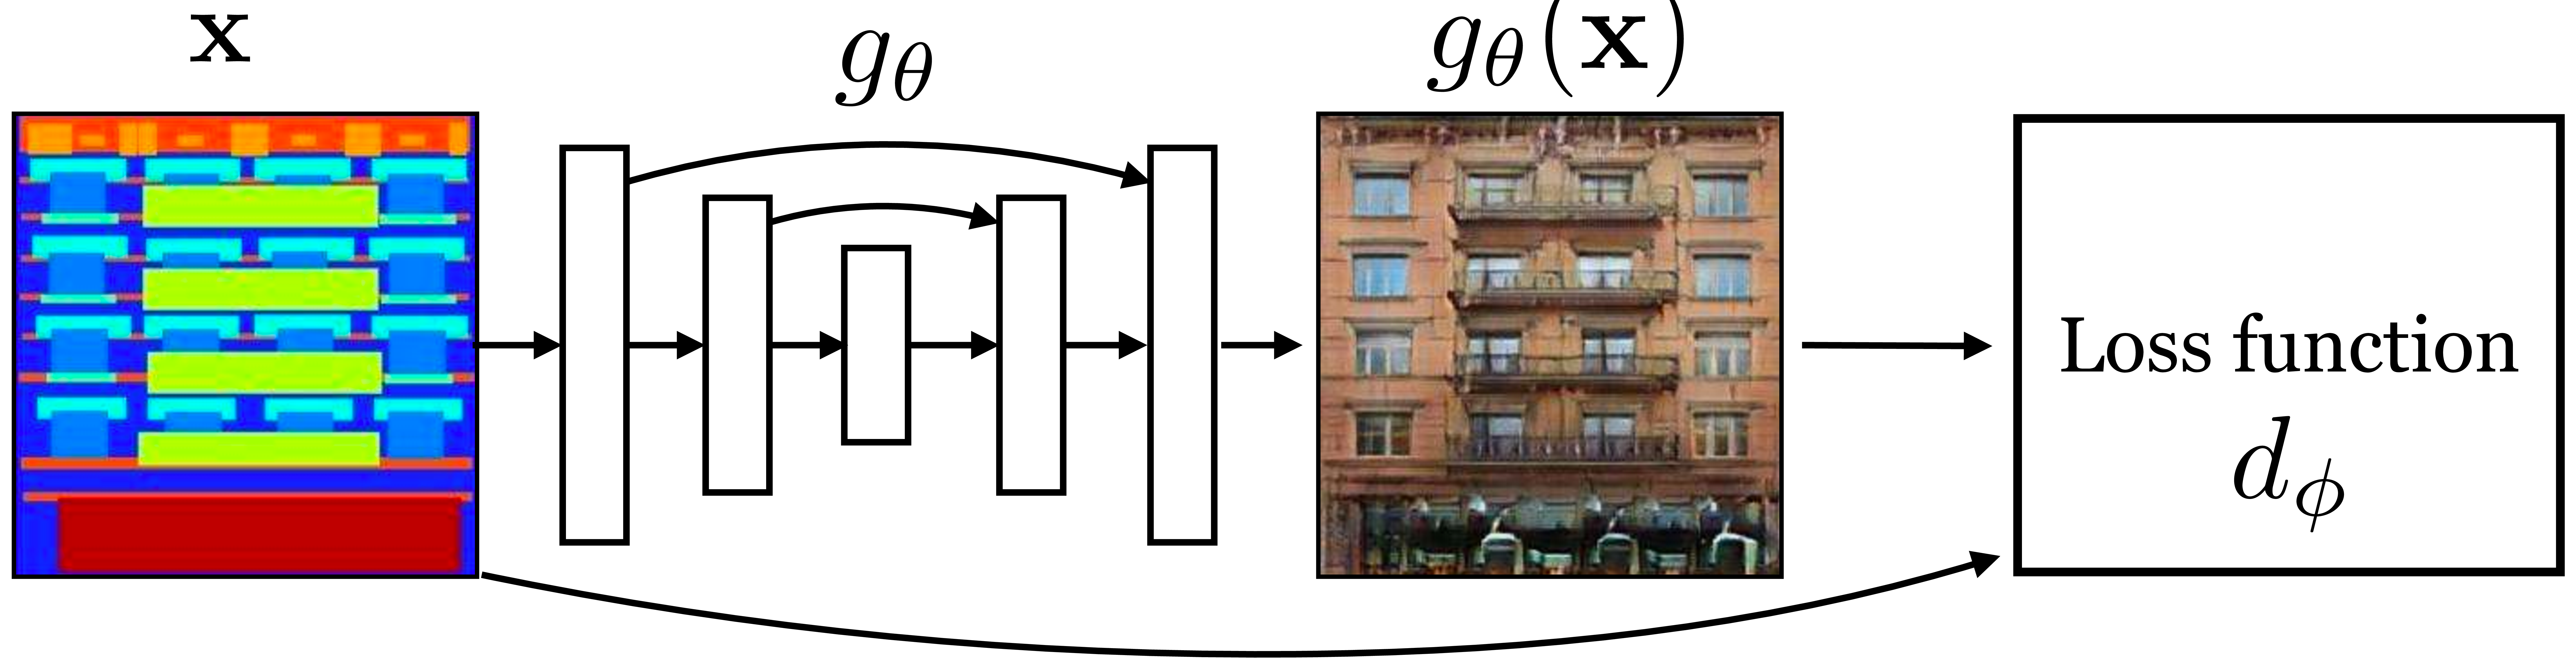
\includegraphics[width=0.9\linewidth]{./figures/conditional_generative_models/cGAN_as_learned_loss.pdf}
    }
    \caption{The discriminator of a GAN as a learned loss function.}
    \label{fig:conditional_generative_models:cGAN_as_learned_loss}
\end{figure}

This loss function adapts to the structure of the data and the behavior of the generator to penalize just the relevant errors the generator is currently making. It can help to also add a conventional regression loss, such as the $L_1$ loss, to stabilize the optimization process, yielding the following objective:
\begin{align}
    \arg\min_G\max_D \mathbb{E}_{\mathbf{z},\mathbf{x},\mathbf{y}} \big[ \log d_{\phi}(\mathbf{x}, g_{\theta}(\mathbf{x},\mathbf{z})) + \log (1 - d_{\phi}(\mathbf{x}, \mathbf{y})) + \norm{g_{\theta}(\mathbf{x}) - \mathbf{y}}_1 \big]\label{eqn:conditional_generative_models:cGAN_objective_plus_L}
\end{align}

Thinking of $d_{\phi}$ as a learned loss function raises new questions: What does this loss function penalize, and how can we control its properties. One of the main levers we have is the architecture of $d_{\phi}$; different architectures will have the capacity, and/or inductive bias, to penalize different kinds of errors. One popular architecture for image-to-image tasks is a \index{PatchGAN}\textbf{PatchGAN} discriminator~\cite{pix2pix2017}, in which we score each \textit{patch} in the output image as real or fake and take the average over patch scores as our total loss:
\begin{align}
    d_{\phi}(\mathbf{x}, \mathbf{y}) = \frac{1}{NM} \sum_{i=0}^N \sum_{j=0}^M d_{\phi}^{\texttt{patch}}(\mathbf{x}[i:i+k,j:j+k], \mathbf{y}[i:i+k,j:j+k]) \label{eqn:conditional_generative_models:patchgan_objective}
\end{align}
where $k \times k$ is the patch size. Notice that this operation is equivalent to the sliding window action of CNN, so $d_{\phi}^{\texttt{patch}}$ can simply be implemented as a CNN that outputs a $2 \times N \times M$ feature map of real-versus-synthetic scores. Naturally, patches can be sampled at different strides and resolutions, depending on the exact architecture of the CNN $d_{\phi}^{\texttt{patch}}$.

The PatchGAN strategy has two advantages over just scoring the whole image as real or synthetic with a classifier architecture: (1) it can be easier to model if a patch is real or synthetic than to model if an entire image is real or synthetic ($d_{\phi}^{\texttt{patch}}$ needs fewer parameters), (2) there are more patches in the training data than their are images. These two properities give PatchGAN discriminators a statistical advantage over whole image discrimatinators (fewer parameters fit to more data). The disadvantage is that the PatchGAN only has the architectural capacity to penalize errors that are observable within a single patch. This can be seen by training models with different discriminator patch sizes and observing the results. We show this in \fig{\ref{fig:conditional_generative_models:patchgan_patch_size_variations}}. %for a conditional GAN trained to map from architectural label maps to building facade images (the label colors indicate whether that region of the image contains a window, door, column, etc.).
\begin{figure}[h!]
    \centerline{
        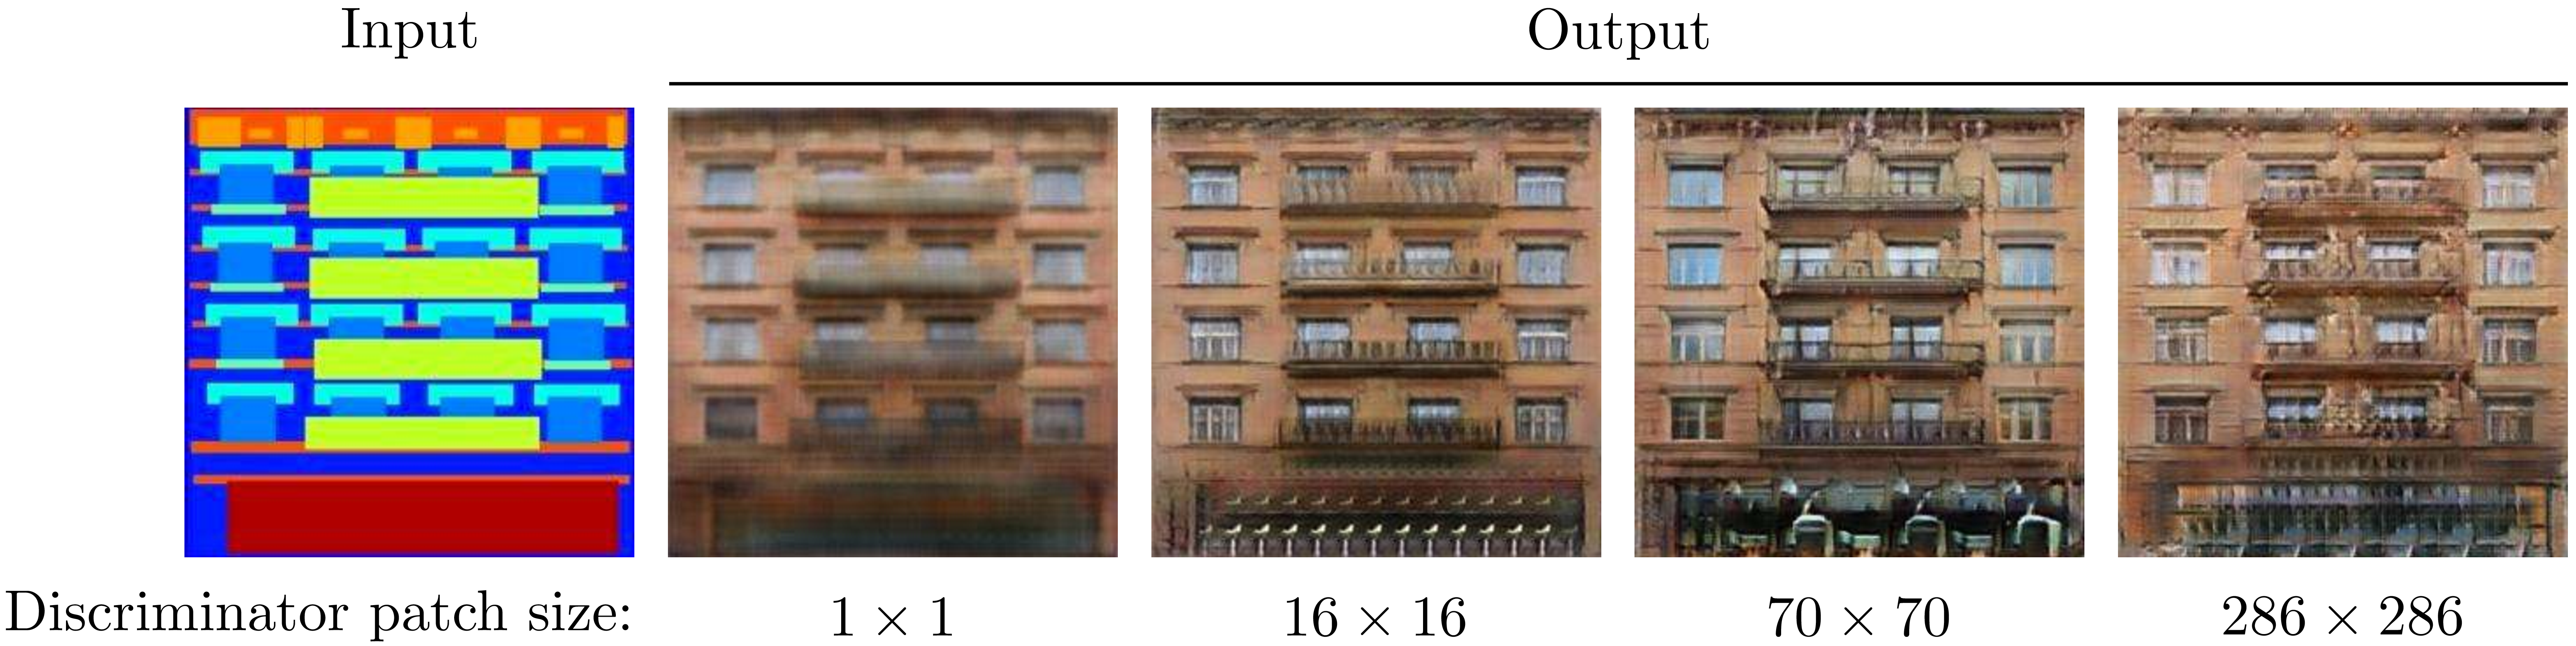
\includegraphics[width=1.0\linewidth]{./figures/conditional_generative_models/patchgan_patch_size_variations.pdf}
    }
    \caption{Varying the receptive field (patch size) of the convolutional discriminator affects what kinds of structure the discriminator enforces. These results are from \cite{pix2pix2017}}.
    \label{fig:conditional_generative_models:patchgan_patch_size_variations}
\end{figure}

A $1\times1$ discriminator can only observe a single pixel at a time and cannot penalize errors in joint pixel statistics such as edge structure, hence the blurry results. Larger receptive fields can enforce higher order patch realism, but cannot model structure larger than the patch size (hence the tiling artifacts that are occur with a period roughly equal to the patch size). Quality degrades with the $286\times286$ discriminator possibly because this disciminator has too hard a task given the limited training data (in any given training set, there are fewer examples of $286\times286$ regions than there are of, say, $70\times70$ regions).

%For example, what would a sketch look like if it were a photo? This problem requires a generative model because the output is structured and uncertain (there are many possible outputs for any one input). This problem requires a conditional model since we are basing the prediction on an input visualization -- a sketch in this example. Therefore, conditional generative models, and in particular conditional GANs, have been shown to be very effective at this task~\cite{pix2pix2017}.

% They can do so according to a few strategies:
% \begin{enumerate}
%     \item Learn a conditional generator function $G: \mathcal{X} \times \mathcal{Z} \rightarrow \mathcal{Y}$, with $Z$ a random variable that makes the mapping stochastic.
%     \item Predict parameters of a density function $f: \mathcal{X} \rightarrow \Phi$, where $\phi \in \Phi$ parameterizes a probability distribution over $\mathcal{Y}$.
% \end{enumerate}
% An example of \#4 is softmax regression, where $\phi$ is the logit vector that parameterizes a categorical distribution over output discrete classes.

%Important considerations are what's a good architecture for generating images and what's a good architecture for the loss function.

\subsection{Unpaired Image-to-Image Translation}
\index{Image-to-image translation!Unpaired}

In the preceding section we saw how to solve image-to-image translation by treating it just like a supervised regression problem, except using a learned loss function given by a GAN discriminator. This approach works great when we have lots of training data pairs $\{\mathbf{x}, \mathbf{y}\}$ to learn from. Unfortunately, very often, paired training data is hard to obtain. For example, consider the task of translating a photo into a Cezanne painting (\fig{\ref{fig:conditional_generative_models:cyclegan_teaser}}):
\begin{figure}[h!]
    \centerline{
        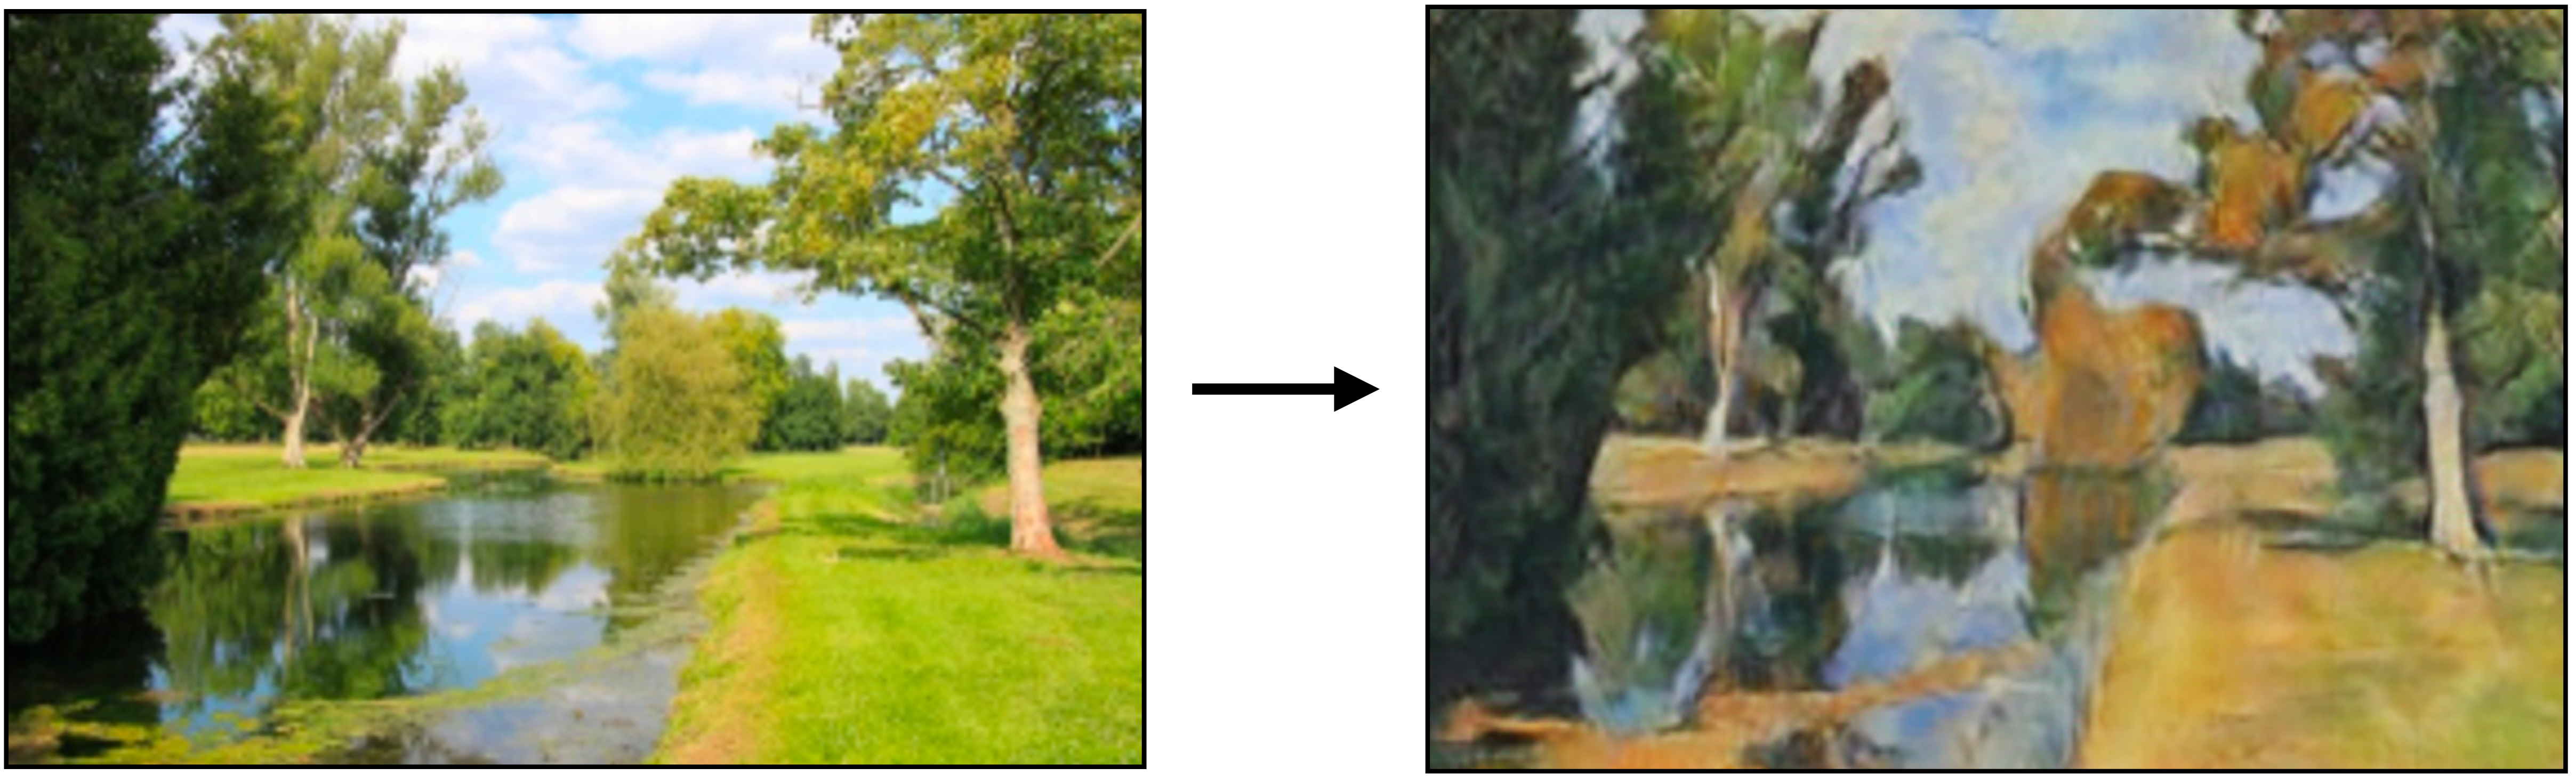
\includegraphics[width=0.6\linewidth]{./figures/conditional_generative_models/cyclegan_teaser.pdf}
    }
    \caption{A style transfer example from the CycleGAN paper~\cite{CycleGAN2017}. \textit{Input photo source}: Alexei A. Efros.}
    \label{fig:conditional_generative_models:cyclegan_teaser}
\end{figure}

The task depicted here is to predict: What would it have looked like if Cezanne had stood at this riverbank and painted it? %The input and output to one algorithm that can do this (CycleGAN~\cite{CycleGAN2017}) is shown below (\fig{\ref{fig:conditional_generative_models:cyclegan_teaser}}):

How could this be done? We can't have solved it with paired training data because, in this setting, paired data is extremely hard to come by. We would have to resurrect Cezanne and ask him to paint for us a bunch of new scenes, one for each photo in our desired training set. But is all that effort really necessary? You and I, as humans, can certainly imagine the answer to the previous question. We know what Cezanne's style looks like and can reason about the changes that would have to occur to make the photo match his style. Dabs of paint would have to replace the photographic pixels, and the colors should take on more pastel tones. We can imagine the necessary stylistic changes because we have seen many Cezanne paintings before, even though we didn't see them paired with a photograph of the exact same scenes. Let's now see how we can give a machine this same ability. We call this setting the \textbf{unpaired translation} setting, and distinguish it from \textbf{paired translation} as indicated in \fig{\ref{fig:conditional_generative_models:paired_vs_unpaired}}.
\begin{figure}[h!]
    \centerline{
        \includegraphics[width=0.7\linewidth]{./figures/conditional_generative_models/paired_vs_unpaired.pdf}
    }
    \caption{(left) An example of paired image-to-image translation (colorization) versus (right) unpaired translation (photo to Cezanne). Figure adapted from \cite{CycleGAN2017}.}
    \label{fig:conditional_generative_models:paired_vs_unpaired}
\end{figure}

It turns out that GANs have a very useful property that makes them well-suited to solving this task. GANs train a mapping from a noise distribution to a data distribution $p(Z) \rightarrow p(X)$. They do this without knowing the pairing between $\mathbf{z}$ and $\mathbf{x}$ values in the training data. Instead this pairing is \textit{emergent}. Which $\mathbf{z}$-vector corresponds to which $\mathbf{x}$ is not predetermined but self-organizes to satisfy the GAN objective (all $\mathbf{z}$-vectors should map to realistic images, and, collectively they should map to the data distribution).

Now consider training a GAN to map from $\mathbf{x}$ to $\mathbf{y}$ values:
\begin{align}
    \arg\min_{\theta}\max_{\phi} \mathbb{E}_{\mathbf{x},\mathbf{y}} \big[ \log d_{\phi}(g_{\theta}(\mathbf{x})) + \log (1 - d_{\phi}(\mathbf{y})) \big] \label{eqn:conditional_generative_models:x_to_y_GAN_learning_problem}
\end{align}
\marginnote{Note that this is a regular GAN objective rather than a conditional GAN, except that we have relabeled the variables compared to \eqn{\ref{eqn:generative_models:GAN_learning_problem}}, with $\mathbf{y}$ playing the role of $\mathbf{x}$ and $\mathbf{x}$ playing the role of $\mathbf{z}$.}[-0.5cm]
Such a GAN would self-organize so that the outputs are realistic $\mathbf{y}$ values and so that different inputs map to different outputs (collectively they must map to the data distribution over possible $\mathbf{y}$ values). No paired supervision is required to achieve this.

Such a GAN may indeed learn the correct mapping from $\mathbf{x}$ to $\mathbf{y}$ values—that's one of the solutions that minimizes the loss—but there are many symmetries in this learning problem, that is, many different mappings achieve equivalent loss. For example, consider that we permute the mapping: if $\{\mathbf{x}^{(i)}, \mathbf{y}^{(i)}\}$ is the true mapping then consider we instead recover $\{\mathbf{x}^{(i)}, \mathbf{y}^{(i+1)}\}$ after learning (circularly shifting at the boundary). This mapping achieves equal loss to the true mapping, under the standard GAN objective (equation [\ref{eqn:conditional_generative_models:x_to_y_GAN_learning_problem}]). This is because any permutation in the mapping does not affect the output \textit{distribution}, and the GAN objective only cares about the output distribution.

Put another away, the GAN discriminator is different than a normal loss function. Rather than checking if the output matches a target \textit{instance} (that $g_{\theta}(\mathbf{x}^{(i)})$ matches $\mathbf{y}^{(i)})$, it checks if the output is part of an admissible set, that is, the set of things that look like realistic $\mathbf{y}$ values. This property makes GANs perfect for working with unpaired data, where we don't have instance-level supervision but only have set-level superversion.\marginnote{We call this \textbf{unpaired} learning rather than unsupervised because we still have supervision in the form of labels indicating which \textit{set} each datapoint belongs to. That is, we know whether each image is an $\mathbf{x}$ or a $\mathbf{y}$.}[-0.8cm]

So, a regular GAN objective, applied to mapping from $X$ to $Y$, solves the unpaired translation problem, but it does not distinguish between the correct mapping and the many other mappings that achieve the same output distribution. To break the symmetry we need to add additional constraints or inductive biases. One that works especially well is \index{Cycle-consistency}\textbf{cycle-consistency}, which was introduced in this context by CycleGAN~\cite{CycleGAN2017}, DualGAN~\cite{yi2017dualgan}, and DiscoGAN~\cite{kim2017learning}, which are all essentially the same model. The idea of cycle-consistency is that if we translate from $X$ to $Y$ and then translate back (from $Y$ to $X$) we should arrive where we started. Think about translating from English to French, for example. If we translate ``apple'' to French, ``apple''$\rightarrow$``pomme,'' and then translate back, ``pomme''$\rightarrow$``apple,'' we arrive where we started.\footnote{In natural language processing, the idea of cycle-consistency is known as \textbf{backtranslation}.} We can check the quality of a translation system, for a language we are unfamiliar with, by using this trick. If translating back does not return the word we started with then something went wrong with the translation model. This is because we expect language translation to be roughly one-to-one: for each word in English there is usually an equivalent word in French. Cycle-consistency losses are regularizers that encourage a learned mapping to be roughly one-to-one. The cycle-consistency losses from CycleGAN are simply:
\begin{align}
    \mathcal{L}_{\texttt{cyc}}(\mathbf{x};g_{\theta},f_{\psi}) & = \norm{\mathbf{x} - f_{\psi}(g_{\theta}(\mathbf{x}))}_1 \\
    \mathcal{L}_{\texttt{cyc}}(\mathbf{y};g_{\theta},f_{\psi}) & = \norm{\mathbf{y} - g_{\theta}(f_{\psi}(\mathbf{y}))}_1
\end{align}
Adding this loss to \eqn{\ref{eqn:conditional_generative_models:x_to_y_GAN_learning_problem}} yields the complete CycleGAN objective:
\begin{align}
    \arg\min_{\theta,\psi}\max_{\phi} \mathbb{E}_{\mathbf{x},\mathbf{y}} \big[ \log d_{\phi}^{Y}(g_{\theta}(\mathbf{x})) + \log (1 - d_{\phi}^{Y}(\mathbf{y})) + \norm{\mathbf{x} - f_{\psi}(g_{\theta}(\mathbf{x}))}_1 + \\
        \log d_{\phi}^{X}(f_{\psi}(\mathbf{y})) + \log (1 - d_{\phi}^{X}(\mathbf{x})) + \norm{\mathbf{y} - g_{\theta}(f_{\psi}(\mathbf{y}))}_1 \big]
\end{align}
This model translates from domain $X$ to domain $Y$ and back, such that the outputs in domain $Y$ look realistic according to a domain $Y$ discriminator, and vice versa for domain $X$, \textit{and} the mappings are cycle-consistent: one complete cycle from $X$ to $Y$ and back should arrive where it started (and, again, vice versa). A diagram for this whole process is given in \fig{\ref{fig:conditional_generative_models:cyclegan_schematic}}:
\begin{figure}[h!]
    \centerline{
        \includegraphics[width=1.0\linewidth]{./figures/conditional_generative_models/cyclegan_schematic.pdf}
    }
    \caption{CycleGAN schematic. Figure derived from \cite{CycleGAN2017}.}
    \label{fig:conditional_generative_models:cyclegan_schematic}
\end{figure}

The cycle-consistency losses encourage that the translation is a one-to-one function, and thereby reduce the number of valid solutions. This is a good idea when the true solution is indeed one-to-one, as is often the case in translation problems. However, other symmetries still exist and may confound methods like CycleGAN: if we permute the correct $X$-to-$Y$ mapping and apply the inverse permutation to the $Y$-to-$X$ mapping, then CycleGAN will still be satisfied but the mapping will now be incorrect.


\section{Concluding Remarks}
Many problems in vision can be phrased as structured prediction, and conditional generative models are a great approach to these problems. They provide a unified and simple solution to a diverse array of problems. A current trend in computer vision (and all of artificial intelligence) is to replace bespoke systems for specific kinds of structured prediction—object detectors, image captioning systems, and so on—with general-purpose conditional generative models. This is one reason why this book does not focus much on special-purpose systems that solve specific problems in vision—because the trend is toward general-purpose modeling tools.